\documentclass{beamer}

\usepackage{graphicx}
\usepackage{tikz}
\usetikzlibrary{shapes.callouts}
\usepackage{multirow}

%\usetheme{AnnArbor}
%\usetheme{Antibes}
%\usetheme{Bergen}
%\usetheme{Berkeley}
%\usetheme{Berlin}
%\usetheme{Boadilla}
%\usetheme{boxes}
%\usetheme{CambridgeUS}
%\usetheme{Copenhagen}
%\usetheme{Darmstadt}
%\usetheme{default}
%\usetheme{Frankfurt}
%\usetheme{Goettingen}
%\usetheme{Hannover}
%\usetheme{Ilmenau}
%\usetheme{JuanLesPins}
%\usetheme{Luebeck}
%\usetheme{Madrid}
%\usetheme{Malmoe}
%\usetheme{Marburg}
%\usetheme{Montpellier}
%\usetheme{PaloAlto}
%\usetheme{Pittsburgh}
%\usetheme{Rochester}
%\usetheme{Singapore}
%\usetheme{Szeged}
%\usetheme{Warsaw}

\title[EAE105A]{EAE105A \\ Introducci\'on a la Econom\'ia}

\subtitle[Mercado Laboral y Desempleo]{Mercado Laboral y Desempleo}

\institute[PUC]{Instituto de Econom\'ia\\
Pontificia Universidad Cat\'olica de Chile}

\date[$\:$]

\subject{Mercados y Demanda}

\AtBeginSection[]{
\begin{frame}<beamer>{Contenidos}
\tableofcontents[currentsection, currentsubsection]
\end{frame}}

\begin{document}
\maketitle

\begin{frame}
\frametitle{Introducci\'on y motivaci\'on inicial}
\begin{itemize}
\setlength\itemsep{1.4em}
\item Un aspecto crucial de una econom\'ia, es su capacidad de unir trabajadores con el resto de los factores de producci\'on.\\
\item Dicho enlace dista de ser perfecto. Existe el desempleo.
\item El estudio del desempleo se puede dividir en dos partes:\\
\begin{itemize}
\setlength\itemsep{0.6em}
\item[-] Desempleo de largo plazo.
\item[-] Desempleo de corto plazo.
\end{itemize}
\item En esta secci\'on, prestamos atenci\'on a la medici\'on del desempleo de largo plazo.
\end{itemize}
\end{frame}

\begin{frame}
\frametitle{Medici\'on del desempleo}
\begin{itemize}
\setlength\itemsep{1.0em}
\item \textbf{Desempleado}: De acuerdo a la definici\'on de la OMT, desempleado es todo aquel que:\\
\vspace{2mm}
\begin{itemize}
\setlength\itemsep{1.0em}
\item[1.] No ha trabajado a sueldo o bajo auto-empleo durante un per\'iodo de referencia.
\item[2.] Estuvo disponible para trabajar en el per\'iodo de referencia.
\item[3.] Busc\'o trabajo activamente en el per\'iodo de referencia.
\end{itemize}
\item \textbf{Empleado}: De acuerdo a la definici\'on de la OMT, empleado es todo aquel que:
\vspace{2mm}
\begin{itemize}
\item[1.] Trabaj\'o durante el per\'iodo de referencia.
\end{itemize}
\end{itemize}
\end{frame}

\begin{frame}
\frametitle{Medici\'on del desempleo}
\begin{itemize}
\setlength\itemsep{1.0em}
\item Podemos llevar el desglose de la poblaci\'on un paso atr\'as:\\
\begin{center}
\begin{figure}
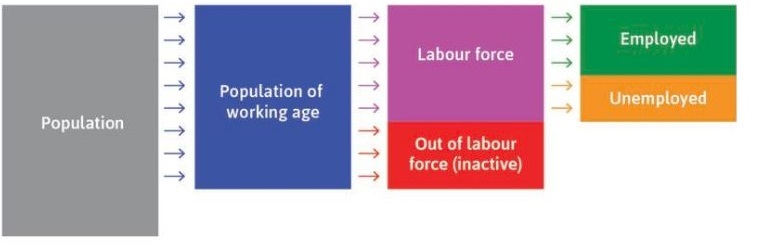
\includegraphics[scale=0.495]{Figuras/Desglose}
\end{figure}
\end{center}
\end{itemize}
\end{frame}

\begin{frame}
\frametitle{Medici\'on del desempleo}
\begin{itemize}
\setlength\itemsep{1.5em}
\item \textbf{Poblaci\'on en edad de trabajo}: Poblaci\'on total menos los ni\~nos y adultos mayores.
\item \textbf{Fuerza laboral}: Poblaci\'on total de trabajadores activos (empleados+desempleados).
\item \textbf{Inactivos}: Individuos que no trabajan y no buscan activamente trabajo.  
\end{itemize}
\end{frame}

\begin{frame}
\frametitle{Medici\'on del desempleo - Estad\'isticos laborales}
\begin{itemize}
\setlength\itemsep{1.4em}
\item Existen varios estad\'isticos que arrojan luz sobre la sistuaci\'on del mercado laboral en un instante dado.
\item \textbf{Tasa de participaci\'on}: Muestra la fracci\'on de la poblaci\'on en edad de trabajo que pertenece a la fuerza laboral. 
\small
\begin{equation*}
\begin{aligned}
\text{Tasa de participaci\'on} & \equiv \frac{\text{Fuerza Laboral}}{\text{Poblaci\'on en edad de trabajo}}\\ & \equiv \frac{\text{Empleados}+\text{Desempleados}}{\text{Poblaci\'on en edad de trabajo}}
\end{aligned}
\end{equation*}
\normalsize
\end{itemize}
\end{frame}

\begin{frame}
\frametitle{Medici\'on del desempleo - Estad\'isticos Laborales}
\begin{itemize}
\setlength\itemsep{1.5em}
\item \textbf{Tasa de desempleo}: Fracci\'on de la fuerza laboral desempleada: $$\text{Tasa de desempleo} \equiv \frac{\text{Desempleados}}{\text{Fuerza Laboral}}$$
\item \textbf{Tasa de empleo}: Fracci\'on de la fuerza laboral empleada: $$\text{Tasa de empleo} \equiv \frac{\text{Empleados}}{\text{Poblaci\'on en edad de trabajo}}$$
\item Notar la diferencia en los denominadores. Dos paises con la misma tasa de desempleo pueden tener diferentes tasas de empleo!
\end{itemize}
\end{frame}

%\begin{frame}
%\frametitle{Medici\'on del desempleo - Ejemplo}
%\begin{itemize}
%\setlength\itemsep{1.5em}
%\item Considere el siguiente ejemplo en que se consideran las mediciones promedio del $2000 - 2015$.\\
%\begin{center}
%\begin{figure}
%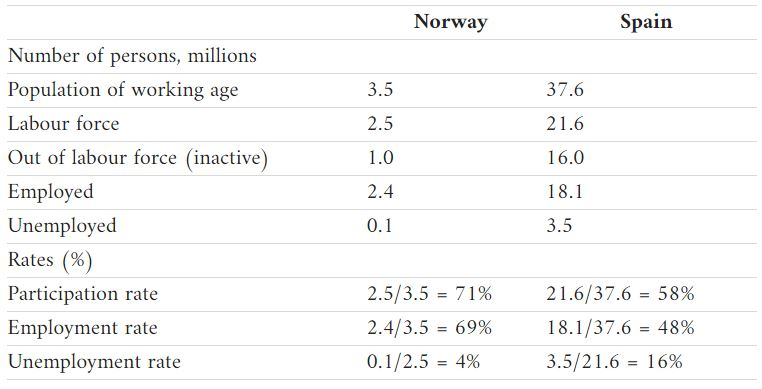
\includegraphics[scale=0.395]{Figuras/Ejemplo1}
%\end{figure}
%\end{center}
%\end{itemize}
%\end{frame}

\begin{frame}
\frametitle{Medici\'on del desempleo}
\begin{itemize}
\setlength\itemsep{1.4em}
\item Es importante enteder los problemas que presenta la tasa de desempleo a la hora de interpretarla.\\
\vspace{2mm}
\begin{itemize}
\setlength\itemsep{0.9em}
\item[-] Los cambios en la fuerza laboral son muy frecuentes.
\item[-] Algunos individuos que reportan buscar empleo podr\'ian no estar buscando arduamente.
\item[-] Algunos individuos que reportan no buscar empleo podr\'ian a\'un estar dispuestos a trabajar.
\item[-] La duraci\'on del desempleo es relevante para fines de pol\'iticas p\'ublicas.
\end{itemize}
\item Existen varias medidas que complementan a la tasa de desempleo y facilitan la interpretaci\'on.
\end{itemize}
\end{frame}

\begin{frame}
\frametitle{Desempleo natural vs desempleo c\'iclico}
\begin{itemize}
\setlength\itemsep{1.5em}
\item Dos aspectos interesantes del gr\'afico anterior:\\
\begin{itemize}
\setlength\itemsep{0.8em}
\item[-] La tasa de desempleo fluctua a lo largo del tiempo.
\item[-] La tasa de desempleo se mantiene siempre por encima de $0$.
\end{itemize}
\item \textbf{Tasa natural de desempleo}: Tasa de desempleo alrededor de la cual el desempleo fluct\'ua en el tiempo.
\item \textbf{Desempleo c\'iclico}: Desviaciones de la tasa de desempleo alrededor del desempleo natural.
\end{itemize}
\end{frame}

\begin{frame}
\frametitle{Desempleo natural}
\begin{itemize}
\setlength\itemsep{1.5em}
\item Hemos visto que en otros mercado el precio se ajusta como para eliminar cualquier exceso de oferta o demanda.
\item Este no resulta ser el caso en el mercado laboral. Estudiaremos dos potenciales explicaciones.\\
\begin{itemize}
\setlength\itemsep{0.8em}
\item[-] Desempleo friccional.
\item[-] Desempleo estructural.
\end{itemize}
\item Tratemos de diseccionar las anteriores.
\end{itemize}
\end{frame}

\begin{frame}
\frametitle{Desempleo friccional}
\begin{itemize}
\setlength\itemsep{1.5em}
\item \textbf{Desempleo friccional}: Desempleo que resulta del proceso de b\'usqueda y apareamiento entre trabajadores y empleadores.
\item Si todos los trabajadores fuesen iguales no existir\'ia desempleo friccional.
\item En la pr\'actica los trabajadores difieren en cuanto a sus habilidades y preferencias laborales. 
\item La informaci\'on sobre los potenciales trabajadores se disemina lentamente en la econom\'ia.
\end{itemize}
\end{frame}

\begin{frame}
\frametitle{Desempleo friccional}
\begin{itemize}
\setlength\itemsep{1.3em}
\item ?`Qu\'e genera el desempleo friccional?
\item La causa m\'as com\'un son los cambios en las demandas relativas por trabajadores entre empresas.\\
\begin{itemize}
\setlength\itemsep{0.7em}
\item[-] Cambios en la demanda de los consumidores de un sector a otro sector.
\item[-] Cambios en los precios relativos de los insumos de un sector con respecto a otro sector.
\end{itemize}
\item El contexto en que opera el mercado laboral afectan el desempleo friccional:\\
\begin{itemize}
\setlength\itemsep{0.7em}
\item[-] El internet facilita el apareamiento entre empleados y empleadores.
\item[-] Programas gubernamentales de difusi\'on de vacantes laborales.
\end{itemize}
\end{itemize}
\end{frame}

\begin{frame}
\frametitle{Desempleo friccional - Ejemplo}
\begin{itemize}
\setlength\itemsep{1.4em}
\item \textbf{Asistencia al desempleado}: Programa gubernamental que assite a los individuos que caen en condici\'on de desempleados.
\item ?`Qu\'e consecuencias supone este tipo de pol\'iticas?\\
\begin{itemize}
\setlength\itemsep{1.0em}
\item[-] Reduce los inconvenientes del desempleo para los individuos que caen en condici\'on de desempleo.
\item[-] Reduce los incentivos a buscar empleo activamente.
\item[-] Aumenta los incentivos a colocar filtros m\'as prolongados en el proceso de contrataci\'on.
\end{itemize}
\item Sin pretender hacerlo, dicha pol\'itica puede terminar aumentando el desempleo friccional.
\end{itemize}
\end{frame}

\begin{frame}
\frametitle{Desempleo estructural}
\begin{itemize}
\setlength\itemsep{1.4em}
\item \textbf{Desempleo estructural}: Desempleo que surge cuando la demanda por trabajadores cae por debajo de la oferta de trabajadores.
\item Tres causas del desempleo estructural:\\
\begin{itemize}
\setlength\itemsep{1.0em}
\item[1.] Salarios m\'inimos.
\item[2.] Sindicatos y colectivos laborales.
\item[3.] Salarios de eficiencia.
\end{itemize}
\end{itemize}
\end{frame}

\begin{frame}
\frametitle{Desempleo estructural - Salarios m\'inimos}
\begin{itemize}
\setlength\itemsep{1.4em}
\item \textbf{Salario m\'inimo}: M\'inimo salario que un empleador puede otorgar a un empleado.
\item La cota sobre los salarios impide que los mismos se ajusten reduciendo el desempleo.
\item Es importante notar que los salario m\'inimos s\'olo tienen efecto sobre una fracci\'on de las interacciones laborales.\\
\begin{itemize}
\item[-] En general, aquellos empleos poco t\'ecnicos.
\end{itemize} 
\end{itemize}
\end{frame}

\begin{frame}
\frametitle{Desempleo estructural - Salarios m\'inimos}
\begin{itemize}
\setlength\itemsep{1.4em}
\item Salario m\'imino.
\begin{center}
\begin{figure}
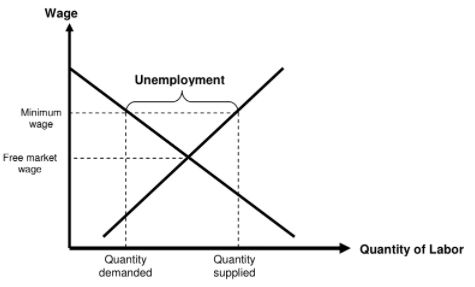
\includegraphics[scale=0.650]{Figuras/Ejemplo3}
\end{figure}
\end{center}
\end{itemize}
\end{frame}

\begin{frame}
\frametitle{Desempleo estructural - Sindicatos y colectivos laborales}
\begin{itemize}
\setlength\itemsep{1.4em}
\item \textbf{Sindicato}: Organizaci\'on de trabajadores que negocia salarios y condiciones laborales con empleadores.
\item La existencia de sindicatos hace que los salarios no correspondan a los del equilibrio competitivo.\\
\begin{itemize}
\item Mayor oferta laboral y menor demanda laboral.
\end{itemize}
\item Los sindicatos pueden ejercer presi\'on a los empleadores mediante huelgas.
\item En general, el poder de un sindicato, depende de la legislaci\'on vigente en la econom\'ia.
\end{itemize}
\end{frame}

\begin{frame}
\frametitle{Desempleo estructural - Salarios eficientes}
\begin{itemize}
\setlength\itemsep{1.4em}
\item \textbf{Teor\'ia salarios eficientes}: Plantea que las empresas aumentan su eficiencia cuando ofrecen un salario por encima del salario competitivo.
\item ?`Qu\'e canales propone la teor\'ia de salarios eficientes?\\
\vspace{2mm}
\begin{itemize}
\setlength\itemsep{0.8em}
\item[1.] Salud y bienestar f\'isico de los empleados.
\item[2.] Menor rotaci\'on en el cuerpo de empleados. 
\item[3.] Contrataci\'on de empleados m\'as calificados.
\item[4.] Mayor esfuerzo de los empleados.
\end{itemize}
\end{itemize}
\end{frame}





\end{document}
